\documentclass[12pt]{report}
\usepackage{float}
\usepackage{CJKutf8}
\usepackage{setspace}
%\usepackage{pinyin}

%==
\usepackage[english]{babel}
\usepackage{amssymb,amsfonts,amsmath,amsthm}
\usepackage{graphicx}
\usepackage{makeidx}
\usepackage{hyperref}
\usepackage[toc,page]{appendix}
%==
\usepackage[a4paper,left=3cm,top=3cm,right=3cm,bottom=3cm,nohead]{geometry}

\usepackage{algorithm}
\usepackage{enumerate}
\usepackage{algpseudocode}

%
% ---- probabilities ----

% ---- others ----
\newtheorem{theorem}{Theorem}[section]
\newtheorem{corollary}{Corollary}[theorem]
\newtheorem{lemma}[theorem]{Lemma}

\doublespacing
\pagestyle{plain}

\begin{document}
\onehalfspacing
%\renewcommand{\baselinestretch}{1.5} 

\begin{titlepage}
\begin{center}

\begin{CJK}{UTF8}{bkai}
\Large{{國立臺灣大學理學院應用數學科學研究所\\碩士論文}}\\
\large{{Institute of Applied Mathematical Science}}\\
\large{College of Science}\\
\Large{{National Taiwan University}}\\
\Large{{Master Thesis}}\\

\hspace*{1cm}~\\
\hspace*{1cm}~\\
\hspace*{1cm}~\\

\Large{遷移學習應用於\\
二維胰臟影像小區塊方式之腫瘤辨識\\
Applying Transfer Learning on \\
2D Patch-Based Healthy Pancreas and Pancreatic Tumor Classification}\\

\hspace*{1cm}~\\
\hspace*{1cm}~\\
\hspace*{1cm}~\\

\Large{楊宛芸\\Wanyun Yang}\\
\hspace*{1cm}~\\
\hspace*{1cm}~\\

\Large{指導教授:王偉仲 教授\\Advisor: Weichung Wang, Ph.D.}\\
\hspace*{1cm}~\\
\hspace*{1cm}~\\

%看要不要"日"
\Large{中華民國 109 年 4 月 (24日)}\\ 
%February, 2020}\\
%\today

\end{CJK}
\end{center}
\end{titlepage}



%\usepackage[a4paper,left=3cm,top=3cm,right=3cm,bottom=2cm,nohead]{geometry}

\doublespacing

\begin{center}
\Large{{Acknowledgement}}\\
\end{center}
I would first like to thank my thesis advisor, professor Weichung Wang. His lab provides rich learning resources and precious opportunities. He consistently allowed this paper to be my own work, but steered me in the right the direction whenever I have difficulties in research. 

I would also like to thank the doctors at National Taiwan University Hospital who were involved in the pancreatic project: Dr. Wei-Chih Liao and Dr. Poting Chen. Without their medical professionalism and advice on research method, the research could not have been successfully conducted. 

I'm glad to thank a excellent research assistant Tinghui Wu of the Academia Sinica as the second reader of this thesis, and I am gratefully indebted to her for her very valuable comments on this thesis. She also kindly helped me for both programming and experiment setting. 

Finally, I must express my very profound gratitude to my parents and to my friends Chunshuo Chen and YuYuan Yuan. At the end of the second semester of master degree, I was stranded at a bottleneck of my research. They provided me with practical support and encouragement throughout my dilemma and through the process of researching and writing this thesis.  This accomplishment would not have been possible without them. Thank you. 

\clearpage

\pagenumbering{roman}
\setcounter{page}{1}

%\doublespacing



%\usepackage[a4paper,left=3cm,top=3cm,right=3cm,bottom=2cm,nohead]{geometry}

\doublespacing
\addcontentsline{toc}{chapter}{Abstract}
\begin{center}
\Large{{Abstract}}\\
\end{center}
Pancreatic cancer is the second most frequent cancer of the digestive system, and artificial intelligence is frequently applied to help doctors with tumor detection. \\

Since all medical images, including pancreas CT, are precious and hard to get, I tried transfer learning on images to improve performance on external dataset. With the help of doctors, I get enough data to train an accurate convolution neural network as source model. In the future I will apply recent model to different datasets, but the AUC performance of classification model decreases when testing on other datasets. My goal is to enhance the performance of model on other dataset. \\

In this paper, I seek to answer the following core question in the context of medical image analysis: how fine-tuning improves the performance on external dataset; how much data we need to get a certain performance. Our experiments consistently demonstrated that, as we get more and more external data, we can get a better prediction result on external data. This paper can help to evaluate how many external data we need to get a satisfying result and help to promote the previous neural network model worldwide. Also, incremental learning was used to evaluate which external scan image (without a manual label) improved the performance most so that we can choose valuable data to label. \\

In this thesis, I found that mixed data method and fine-tuning method can obviously enhance the model performance on external data. The selection method incremental provided can slightly improve the model performance, but overall it doesn't perform better than basic fine-tuning. \\

Key words : Medical Images, Artificial Intelligence, Neural Network, Deep Learning, Transfer Learning


\clearpage

\tableofcontents

%%\listoftables
%%\listoffigures
%%\listofalgorithms

\clearpage

\doublespacing
\pagenumbering{arabic}
\setcounter{page}{1}
\setcounter{tocdepth}{1}


\input{3_Introduction}
\chapter{Methods}
 
\section{Study Design}
\subsection{Prospective or retrospective study}
((5)) \\
XXX 

\subsection{Study goal*}
((6)) \\
\section{Data}
\subsection{Data Source}
((7)) \\
This thesis applies three datasets. All of them are pancreatic CT images.
\begin{itemize}
    \item {\bf National Taiwan University Hospital (ntuh, source data)} \\including both healthy (400) and tumor (400) CT scans. 
    \item {\bf Medical Segmentation Decathlon\cite{simpson2019large} (msd, target data)}\\ including only tumor (281) CT scans. 
    \item {\bf The Cancer Imaging Archive (tcia, target data)}\\ including only healthy (82) CT scans. 
\end{itemize}

\subsection{Eligibility criteria*}
((8 ?)) \\

\subsection{Data Preprocessing}
((9? )) \\
All CT images that contained the pancreas or PC from an individual subject were manually labeled for further model training/validation and testing using an open source software (3D Slicer version 4.8.1). 
Since the pancreas bordered multiple organs/structures and PCs often had an indistinct border with the surrounding tissue, there are inter-observer differences regarding the exact extent of the pancreas and the cancer tumor. Therefore, the labeled pancreas and tumor on the images were checked by the radiologists before further processing and analysis steps. The window width and window level were fixed as 250 Hounsfield unit (HU) and 75 HU, respectively. The images were normalized to [0, 1] by linear interpolation, and the portions that were neither pancreas nor tumor were excluded from further analysis. The images were then cropped into square sub-regions (i.e. 50 $ \times $ 50 patches) using the moving window method on the axial (x-y) plane, starting from the top-left corner and ended at the bottom-right corner. Moving distance was set as half of the patch dimension to generate overlapping patches in order to increase the variation and size of training data. The patches which contained PC were labeled as cancerous, whereas patches that contained only non-cancerous pancreatic parenchyma were labeled as non-cancerous.
((8-10 ignore, 11, 12, 13))
XXX data size?

((8-10 ignore, 11, 12, 13))
\section{Data Partitions*}
\subsection{Sample Size and How It Was Determined}
((Intended sample size and how it was determined))
\subsection{Assign to partitions}
((How data were assigned to partitions; specify proportions))


\section{Model}
\subsection{Detailed description of model}
((Detailed description of model, including inputs, outputs, all intermediate layers and connections)) \\

The CNN model was modified from VGG network12, a neural network widely used in image classification. Weighted binary cross-entropy13 was used as the loss function to solve the  imbalance problem between the number of cancerous and noncancerous patches. Table 1 provides the details of the CNN model, including the layer structures, kernel sizes, channels, and output sizes of the network.
Two callbacks monitoring on validation loss were used during the training process to optimize model performance. All codes were written in Python (version 3.6.8) using Keras (version 2.2.4)14 and Tensorflow (version 1.7.0)15 libraries.

\begin{table}[H]
\centering
\caption{CNN model Structure}
\begin{tabular}{|l|l|l|} 
\hline
Layer (type)              & Output Shape      & Parameter  \\ 
\hline
conv2d 1 (Conv2D)             & (None, 50, 50, 16) &  416 \\
\hline
conv2d 2 (Conv2D)        & (None, 50, 50, 32)                        & 12832        \\
\hline
max pooling2d 1 (MaxPooling2) &  (None, 50, 50, 32) &  0         \\
\hline
conv2d 3 (Conv2D)                                    & (None, 25, 25, 64)                        & 18496                            \\
\hline
conv2d 4 (Conv2D)             & (None, 25, 25, 64) & 36928     \\
\hline
max pooling2d 2 (MaxPooling2)                        & (None, 12, 12, 64)                        & 0                                \\
\hline
conv2d 5 (Conv2D)                                    & (None, 12, 12, 128)                       & 73856                            \\
\hline
conv2d 6 (Conv2D)                                    & (None, 12, 12, 128)                       & 147584                           \\
\hline
max pooling2d 3 (MaxPooling2)                        & (None, 6, 6, 128)                         & 0                                \\
\hline
flatten 1 (Flatten)                                  & (None, 4608)                              & 0                                \\
\hline
dense 1 (Dense)                                      & (None, 32)                                & 147488                           \\
\hline
dropout 1 (Dropout)                                  & (None, 32)                                & 0                                \\
\hline
dense 2 (Dense)                                      & (None, 32)                                & 1056                             \\
\hline
dense 3 (Dense)                                      & (None, 1)                                 & 33 \\
\hline
\end{tabular}
\end{table}

\subsection{Software libraries, frameworks, and packages*}
((Software libraries, frameworks, and packages)) \\
\subsection{Initialization of model parameters*}
((Initialization of model parameters (eg, randomization, transfer learning))) \\



\section{Training*}
\subsection{Training approach}
((Details of training approach, including data augmentation, hyperparameters, number of models trained)) \\
\subsection{Method of selecting the final model}
((Method of selecting the final model)) \\
\subsection{Ensembling techniques, if applicable (ignore)}
((Ensembling techniques, if applicable (ignore))) \\

\section{Evaluation}
This chapter consists of three experiments: basic validation, mix data training and fine tuning. To better observing the result, this thesis use cross validation to distribute training/validation/testing set. 


\subsection{Model performance}
((Metrics of model performance)) \\

\subsubsection{Basic Validation}
In this part, we train model only using target data. We want to find how many patients in target data is needed to build a sufficiently nice model. That means, the AUC of model is larger than 0.8. The table below is the diagram of the number of training/validation/testing set of this experiment. We increase the number of target data to observe the performance of model trained by target data (82, 164, 246, 326 target data).
\begin{table}[H]
\centering
\caption{training/validation/testing set (A) (Basic Validation, 10 folder)}
\begin{tabular}{|l|l|l|l|l|} 
\hline
~            & source H & source T & target H (tcia) & target T (msd)  \\ 
\hline
train        & 0      & 0      & -               & -               \\ 
\hline
validation   & 0       & 0       & -               & -               \\ 
\hline
source test  & 40       & 40       & 0               & 0               \\ 
\hline
target test~ & 0        & 0        & 8               & 28              \\
\hline
\end{tabular}
\end{table}

\begin{table}[H]
\centering 
\caption{training/validation/testing set (B) (10 folder)}
\begin{tabular}{|l|l|l|l|l|} 
\hline
amount of data   & tar H (train) & tar T (train) & tar H (val) & tar T (val)  \\ 
\hline
82        & 17      & 57      & 2               & 6               \\ 
\hline
164   & 33       & 114       & 4               & 13               \\ 
\hline
246  & 50       & 171       & 6               & 19               \\ 
\hline
326 & 66        & 228        & 7               & 25              \\
\hline
\end{tabular}
\end{table}

\subsubsection{Mix Source and Target Data}
In this part, we train model using both source data and target data. We want to find how the number of  patients in target data influences the model performance. The table below is the diagram of the number of training/validation/testing set of this experiment. We increase the number of target data to observe the performance of joint training (82, 164, 246, 326 target data).

\begin{table}[H]
\centering
\caption{training/validation/testing set (Mix Source and Target Data)}
\begin{tabular}{|l|l|l|l|l|} 
\hline
~            & source H & source T & target H (tcia) & target T (msd)  \\ 
\hline
train        & 324      & 324      & -               & -               \\ 
\hline
validation   & 36       & 36       & -               & -               \\ 
\hline
source test  & 40       & 40       & 0               & 0               \\ 
\hline
target test~ & 0        & 0        & 8               & 28              \\
\hline
\end{tabular}
\end{table}

\subsubsection{Transfer Learning}
In this part, first we train model only using source data. Than I use the weight of the previous model as the initial value of training. I train the previous model again using target. The table below is the diagram of the number of training/ validation/ testing set of this experiment. 

\begin{table}[H]
\centering
\caption{training/validation/testing set (A) (Basic Validation, 10 folder)}
\begin{tabular}{|l|l|l|l|l|} 
\hline
~            & source H & source T & target H (tcia) & target T (msd)  \\ 
\hline
train        & 0      & 0      & -               & -               \\ 
\hline
validation   & 0       & 0       & -               & -               \\ 
\hline
source test  & 40       & 40       & 0               & 0               \\ 
\hline
target test~ & 0        & 0        & 8               & 28              \\
\hline
\end{tabular}
\end{table}

\begin{table}[H]
\centering
\caption{training/validation/testing set (B) (10 folder)}
\begin{tabular}{|l|l|l|l|l|} 
\hline
amount of data   & tar H (train) & tar T (train) & tar H (val) & tar T (val)  \\ 
\hline
82        & 17      & 57      & 2               & 6               \\ 
\hline
164   & 33       & 114       & 4               & 13               \\ 
\hline
246  & 50       & 171       & 6               & 19               \\ 
\hline
326 & 66        & 228        & 7               & 25              \\
\hline
\end{tabular}
\end{table}

\subsection{Statistical measures of significance and uncertainty*}
((Statistical measures of significance and uncertainty (eg, confidence intervals))) \\
\subsection{Robustness or sensitivity analysis*}
((Robustness or sensitivity analysis)) \\
\subsection{Methods for explainability or interpretability*}
((Methods for explainability or interpretability (eg, saliency maps) and how they were validated)) \\
\subsection{Validation or testing on external data(ignore)}
((Validation or testing on external data(ignore))) \\





\subsection{Area under the Receiver Operating Characteristic Curve (AUC)?}
A receiver operating characteristic curve, or ROC curve, is a graphical plot that shows the diagnostic ability of a binary classifier system as its predict threshold is varied. The area under the receiver operating characteristic curve is a common criteria to evaluate model performance, not depending on patient threshold. We use AUC in our this thesis. 


\subsection{Transfer Learning and Fine-Tuning?}
In real-world applications, the assumption that the training and future data must be in the same feature space and have the same distribution may not hold. In such cases, knowledge transfer, if done successfully, would highly improve the performance of learning by avoiding much expensive data-labeling efforts. In medical image research, patient data and label is precious and hard to get. Transfer learning has emerged as a new learning framework to solve this problem. Since the target data is labeled, the thesis use fine-tuning to enhance the prediction performance.\cite{pan2009survey}

\subsection{Cross Validation?}
Cross-validation is any of various similar model validation techniques for assessing how the results of a model will generalize to an independent data set.One wants to estimate how accurately a predictive model will perform in practice. The goal of cross-validation is to test the model's ability to predict new data that was excluded from training data, in order to deal with problems like overfitting or selection bias.
\\
Take 5-folder cross validation as an example. There are 400 healthy ntuh data. First we split it into 5 groups (80 data for each group) and take them as test set. 90 percent of the remained data is the training data while 10 percent is the validation data. (Figure 3.1)

\begin{figure}[H]
    \hfil
    \begin{minipage}[t]{0.9\textwidth}
        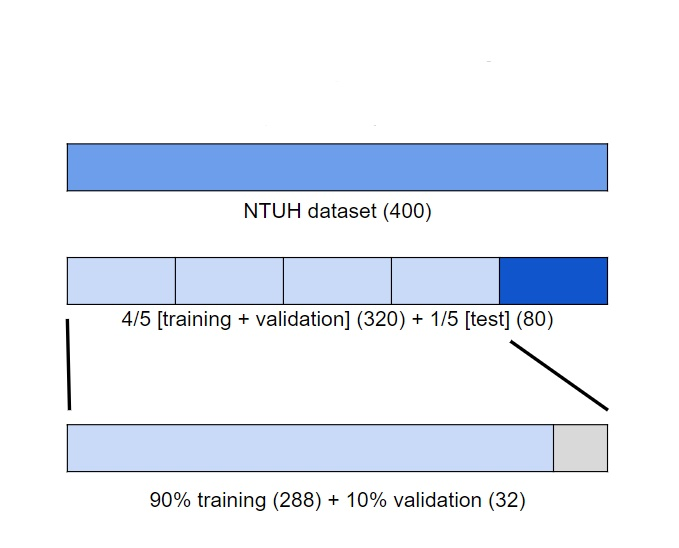
\includegraphics[width=\textwidth]{fig/cross.png}
        \caption{\label{fig:parallel1} training/validation/testing set distribution}
    \end{minipage}
    \hfil
\end{figure}



\chapter{Experiments}
There are 8 experiments in this thesis which can be classified into four parts: basic models, mixed data model, fine-tuning models, and increment fine-tuning models. In the first part, I train models in order to compare with other experiments and choose some parameters. In mixed-data part, I try to train models using both source and target data. When it comes to fine-tuning part, I use target data to fine-tune source model. Finally, I try to add target data gradually into fine-tuned model.

\section{Cross Validation}
I use cross validation to validate my model and divide training/validation/testing sets. Cross validation is validation techniques for assessing how the results of a model will generalize to an independent dataset and estimating how accurately a predictive model will perform in practice. I divide dataset into 10 subsets. Then I choose one to be testing set while the rest part is training set and validation set. For the rest 9 subset, I choose 10 \% to be validation set and the rest 90 \% is training set. The two tables below shows how we divide training/validation/testing sets for source data and target data.


\begin{figure}[H]
    \hfil
    \begin{minipage}[t]{0.9\textwidth}
        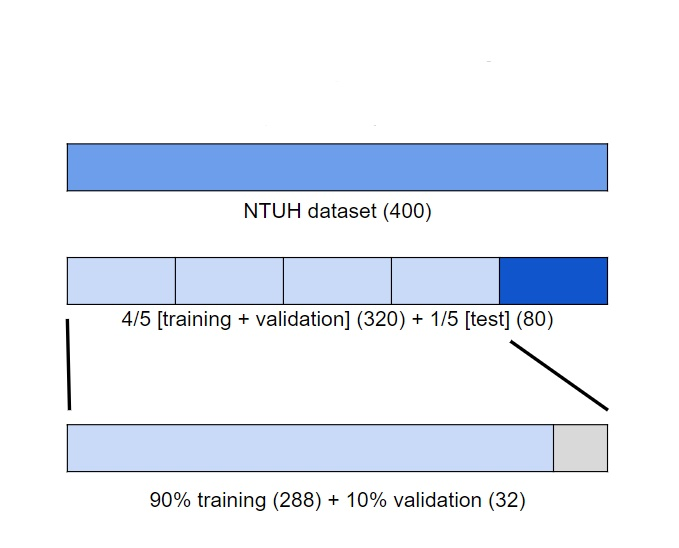
\includegraphics[width=\textwidth]{fig/cross.png}
        \caption{\label{fig:parallel1} AUC for mixed Source Data and Target Data}
    \end{minipage}
    \hfil
\end{figure}
 
 \begin{table}[H]
\centering
\caption{training/validation/testing set (10 folder)}
\begin{tabular}{|l|l|l|l|l|} 
\hline
~            & source H & source T & target H (tcia) & target T (msd)  \\ 
\hline
train        & 330      & 382      & -               & -               \\ 
\hline
validation   & 37       & 42       & -               & -               \\ 
\hline
source test  & 41       & 47       & 0               & 0               \\ 
\hline
target test~ & 0        & 0        & 8               & 18              \\
\hline
\end{tabular}
\end{table}
\begin{table}[H]
\centering 
\caption{training/validation/testing set (B) (10 folder)}
\begin{tabular}{|l|l|l|l|l|} 
\hline
amount of data   & tar H (train) & tar T (train) & tar H (val) & tar T (val)  \\ 
\hline
40       & 11      & 25      & 1               & 3               \\ 
\hline
80 & 22       & 50       & 2               & 6               \\ 
\hline
120 & 34       & 74       & 4               & 8               \\ 
\hline
160 & 45        & 99        & 5               & 11              \\
\hline
200 & 56       & 125       & 6               & 14               \\ 
\hline
\end{tabular}
\end{table}
 ~\\
\section{Basic Models}
In this part, I train models in order to compare with other experiments and choose parameters for other experiments.
\subsection{Train Models Using Only Source Data (B1)}
First, I want to calculate the prediction results if the model is only consider about source data. The results will compare with other experiment results to see how much other methods will improve. The amount of target data fixes 0.
\subsection{Train Models Using Only Target Data (B2)}
I want to calculate the prediction results if the model is only consider about target data. I want to know if how much data is needed to get a sufficiently nice model. The amount of target data varies from 40 to 200.
\subsection{Choose the Number of Fixed Layers in Fine-tuning Experiments (B3)}
All experiments in this thesis use a simplified VGG model for training, however it's better to fix some layers since the target dataset is small for fine-tuning. The goal of this experiment is to find the number of fixed layers in fine-tuning experiments. The amount of target data fixes 200.
~\\
\section{Mixed Data Models}
\subsection{Mixed Data Models (M1)}
In this part, we mixed source and target data to train model. The amount of target data varies from 40 to 200 while the amount of source data fixed.
~\\
\section{Fine-Tuning Models}
\subsection{Fine-Tuning Models (F1)}
In this part, I fine-tuned the model trained in (B1) using target data. I fixed the first three layers in this experiments and use target data to modify the rest layers. The amount of target data varies from 40 to 200.
~\\
\section{Increment Fine-Tuning Models}
Suppose we get an unlabeled target dataset, we want to first label some data that best improve the model performance and use them to fine-tune model. If the AUC performance is not good enough, we need to repeat all steps and fine-tune model using another selected dataset.

\subsection{AIFT Selection Method}
AIFT selection method is applied in increment learning. It calculate the entropy and diversity of the patch-based prediction result of each patient data, and select the data that has the maximum entropy and diversity. For each unlabeled patient data, first I split it into patch-based data. Then use the model generated by source data to predict each patch and get a list of prediction results. Secondly, if the mean value of the list is higher than 0.5, choose the top quarter of list. Otherwise choose the last quarter of list. Then calculate the entropy and diversity of the prediction list. Finally choose a set of patient data that has the highest entropy and diversity and label them. 

\subsection{Fine-tuning Using Selected/Random Target Data (S1/R1)}
This experiment is applied to observe the AUC performance and validate if the selection method AIFT works compared to random selection. We replace the select method to random selection to valid that the selection method really works. 

\subsection{Fine-tuning Using Different Amount of Target data (S2/R2)}
We gradually add selected subset of target data until all target data is used to observe the AUC performance. The amount of target data varies from 40 to 200.

\subsection{Fine-tuning Using Selected/Random Target Data with 66 epochs (S3/R3)}
This experiment is the same as S1/R1 except the number of epochs. I reduce the number of epochs so that the calculation cost is the same as basic fine-tuning method. 
\chapter{Results}
In order to observe the patch-based and patient-based AUC performance, 10-folder cross validation is applied to validate all the experiments .

\section{Model performance}
\subsection{Performance metrics for optimal model}
((Performance metrics for optimal model(s) on all data partitions)) \\

\subsubsection{Basic Validation}
In this experiment, the AUC of experiments increases as the number of training data grows. But the AUC is not high enough for practical use.
\begin{figure}[H]
    \hfil
    \begin{minipage}[t]{0.9\textwidth}
        \includegraphics[width=\textwidth]{fig/A.png}
        \caption{\label{fig:parallel1} AUC for Basic Validation}
    \end{minipage}
    \hfil
\end{figure}
\subsubsection{Mix Source Data and Target Data}
In this experiment, with the help of source data, the AUC of experiments increases as the number of target data grows. The performance increases most when the number of target data is small.
\begin{figure}[H]
    \hfil
    \begin{minipage}[t]{0.9\textwidth}
        \includegraphics[width=\textwidth]{fig/B.png}
        \caption{\label{fig:parallel1} AUC for Mix Source Data and Target Data}
    \end{minipage}
    \hfil
\end{figure}
\subsubsection{Fine Tuning}
In this experiment, I try two methods: fine-tuning with no layer fix and with 3 layers fixed. The AUC of experiments increases as the number of target data grows. The performance of 3 layer-fixed experiment is slightly better than 0 layer-fixed experiment.
\begin{figure}[H]
    \hfil
    \begin{minipage}[t]{0.9\textwidth}
        \includegraphics[width=\textwidth]{fig/C.png}
        \caption{\label{fig:parallel1} AUC for Fine Tuning (fix 0 layer)}
    \end{minipage}
    \hfil
\end{figure}
\begin{figure}[H]
    \hfil
    \begin{minipage}[t]{0.9\textwidth}
        \includegraphics[width=\textwidth]{fig/D.png}
        \caption{\label{fig:parallel1} AUC for Fine Tuning (fix 3 layer)}
    \end{minipage}
    \hfil
\end{figure}

\subsection{Estimates of diagnostic accuracy and their precision*}
((Estimates of diagnostic accuracy and their precision (such as 95 percent confidence intervals))) \\
\subsection{Failure analysis*}
((Failure analysis of incorrectly classified cases)) \\



\chapter{Discussion}
\section{Limitations} 
((Study limitations, including potential bias, statistical uncertainty, and generalizability)) \\
Since the target data is composed of two dataset: MSD dataset and TCIA dataset, the distribution of two datasets might be different, so the model performance may decrease because of the reason. Also, since the number of data is not large enough, the outliers shows up in cross validation experiments. 

\section{Implications for practice*}
((Implications for practice, including the intended use and/or clinical role)) \\

\section{Future Work?}
We can try different fine-tuning details of AIFT method. It's possible to increase the performance on target data. 

\chapter{Other*}
\section{Information}

\subsection{Registration number and name of registry}
\subsection{Where the full study protocol can be accessed}
\subsection{Sources of funding and other support; role of funders}




\printindex


\bibliographystyle{alpha}
\bibliography{mybib}

%\appendix
%\begin{appendices}
% 	\chapter{Proof for example}
% 	\section{title}
% 	Here we consider the case of $q= 12289 $, $k=3$.
% 	The input $U,V$ satisfies the following condition.
% 	\begin{center}
% 		$V = V_0+V_1 \cdot 2^{12} + V_2 \cdot 2^{24}$ and
% 		$U = U_0 + U_1 \cdot 2^{12} $\\
% 	\end{center}
	
	
% 	where 
% 	$0 \leq V_0 < 2^{12}$,
% 	$0 \leq V_1 < 2^{12}$,
% 	$0 \leq V_2 < 2^{6}$,
% 	$0 \leq U_0 < 2^{12}$, and 
% 	$0 \leq U_1 < 2^{4}$ 
% 	%
% 	\begin{center}
% 		$A = \texttt{K-RED}(U)  = 3 U_0 - U_1$ and
% 		$B = \texttt{K-RED2x}(V)  = 9 V_0 - 3 V_1 + V_2$ 
% 	\end{center}

	
	
%\end{appendices}



\end{document}